\documentclass[10pt, a4paper]{article}

\usepackage{algorithm2e}
\usepackage{graphicx}
\usepackage{lscape}

\begin{document}

\title{Wordladders: CS211 Assignment 1}
\date{October 22, 2012}
\author{Samuel B Sherar (sbs1)}

\maketitle
\newpage

\tableofcontents

\newpage

\section{Abstract}

For this assignment, I was asked to create a program which would create and manipulate word ladders. The two methods I have implemented are for generating a wordladder from a given word and the amount of changes; and discovery, which found the shortest path between two given words. In this document, I will go over my design, implementation and testing of the algorithms and data structures, and explain how and why I used certain methods.

\section{UML Diagrams}

\subsection{Use Case Diagram}

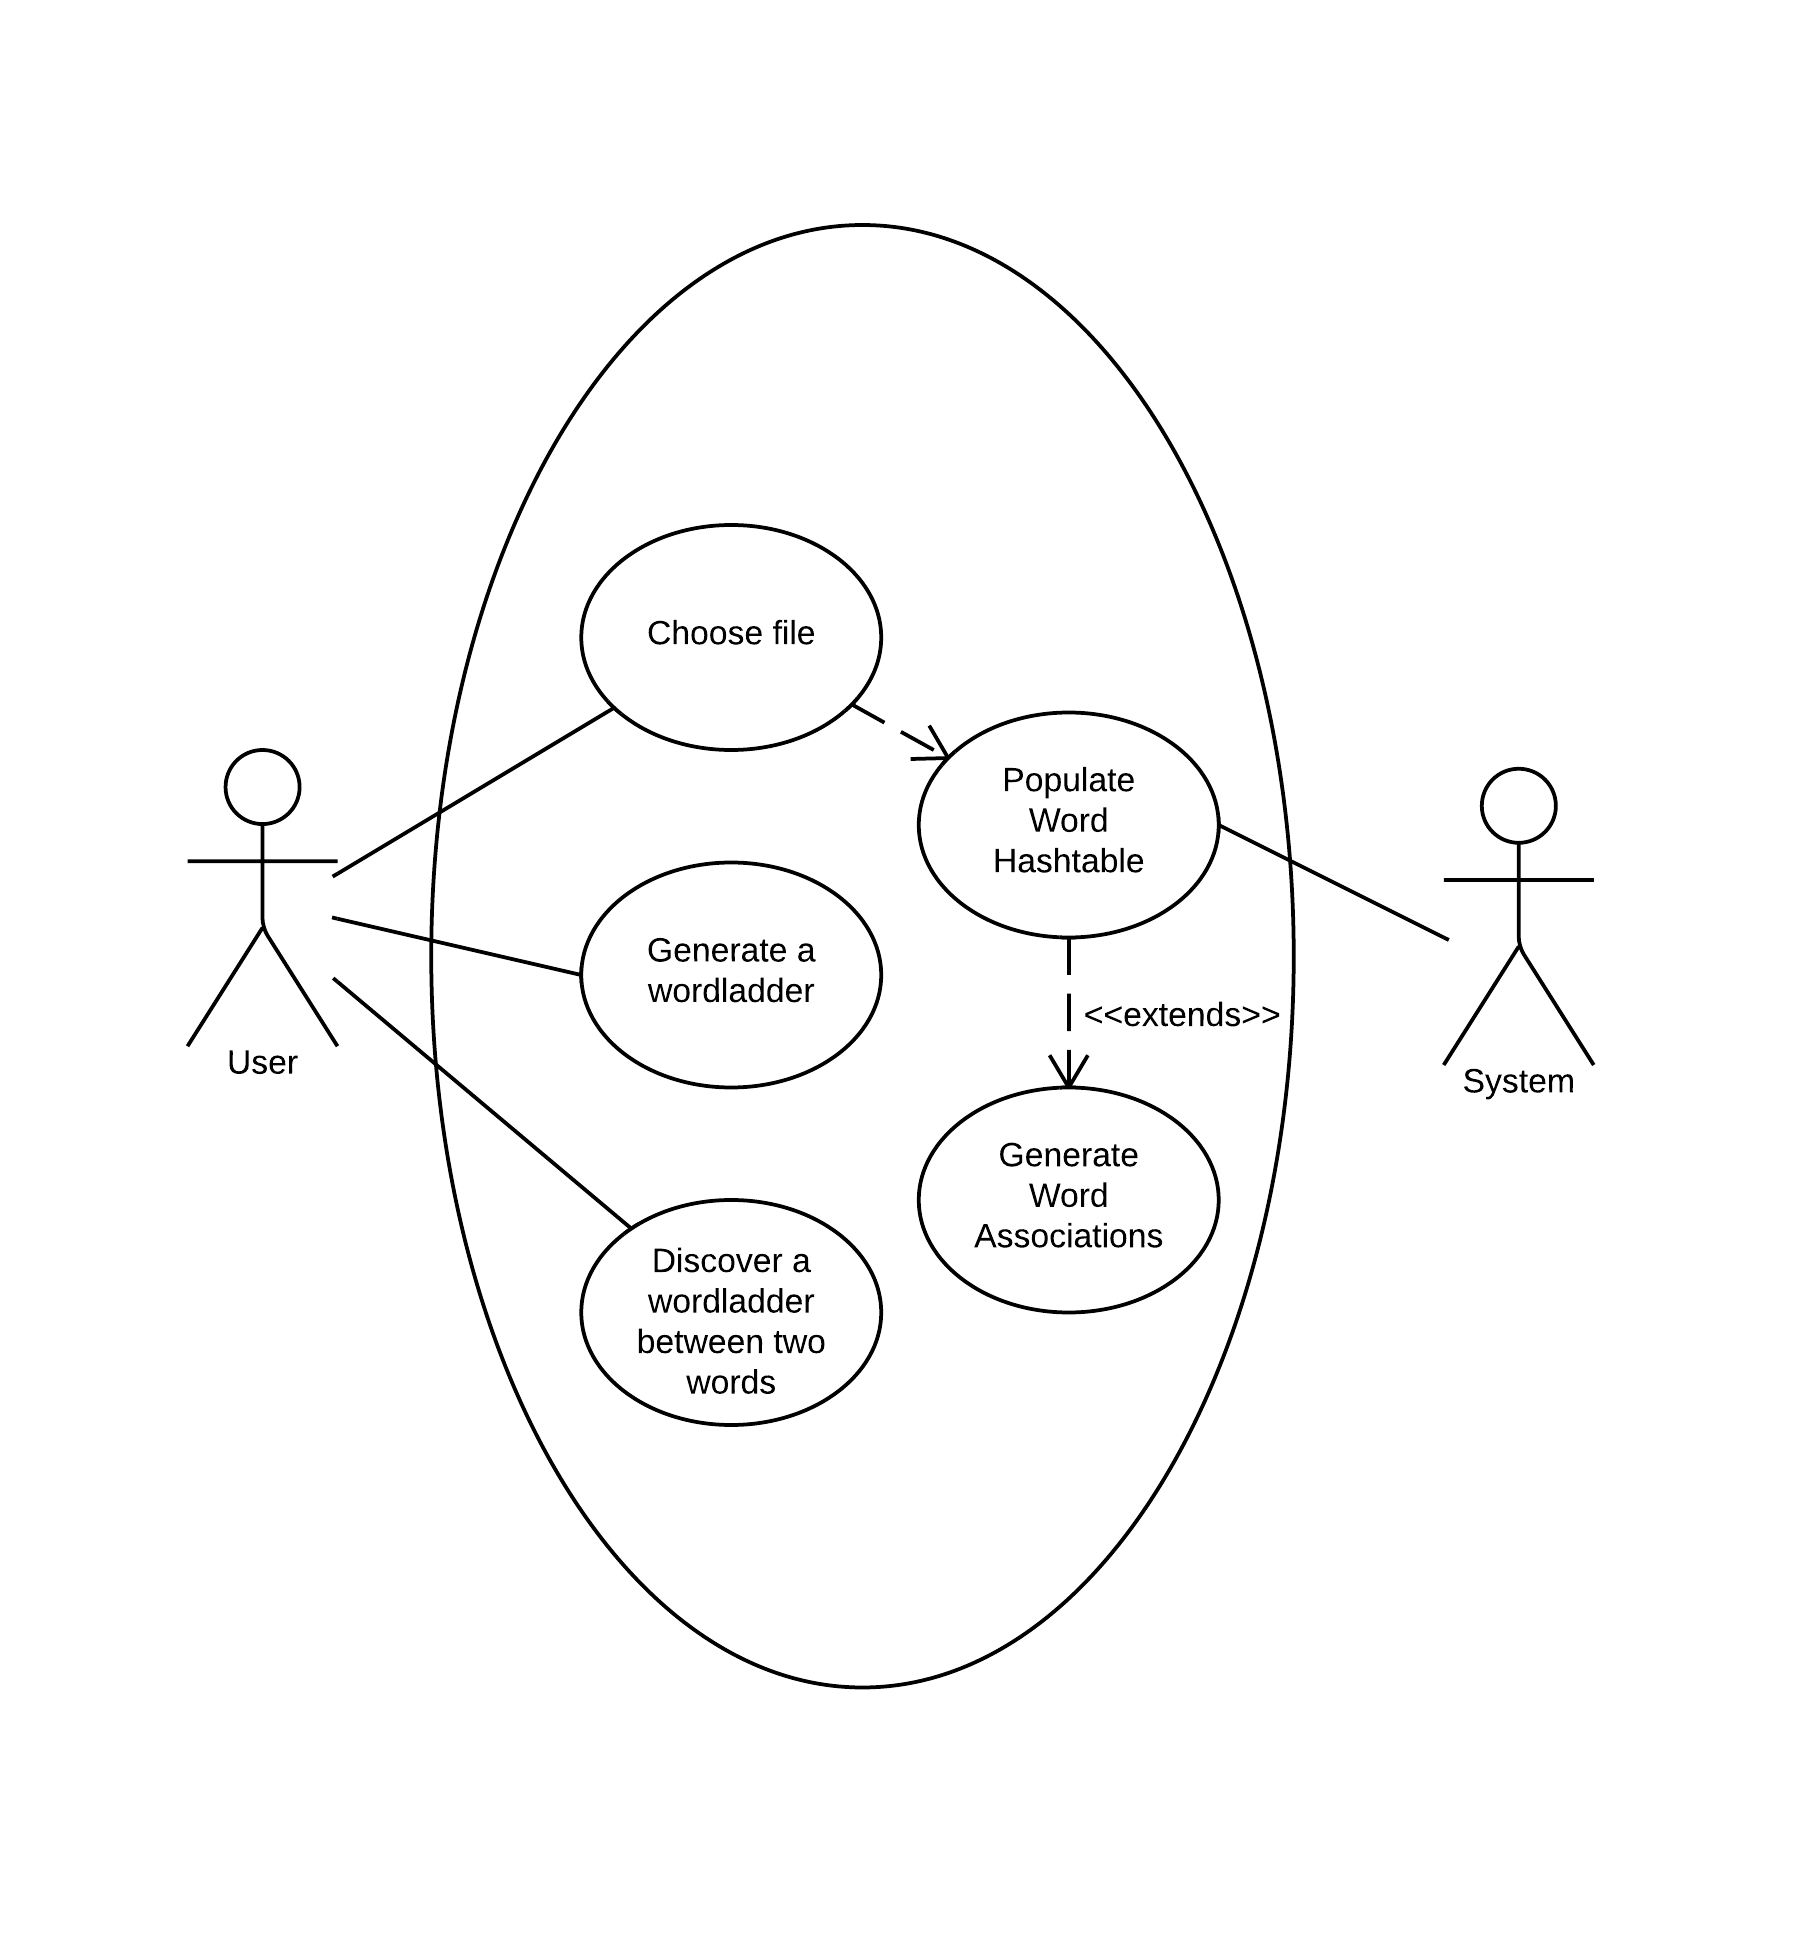
\includegraphics{./images/usecase.png}

\subsection{Class Diagrams}
\hspace*{-1.5in}
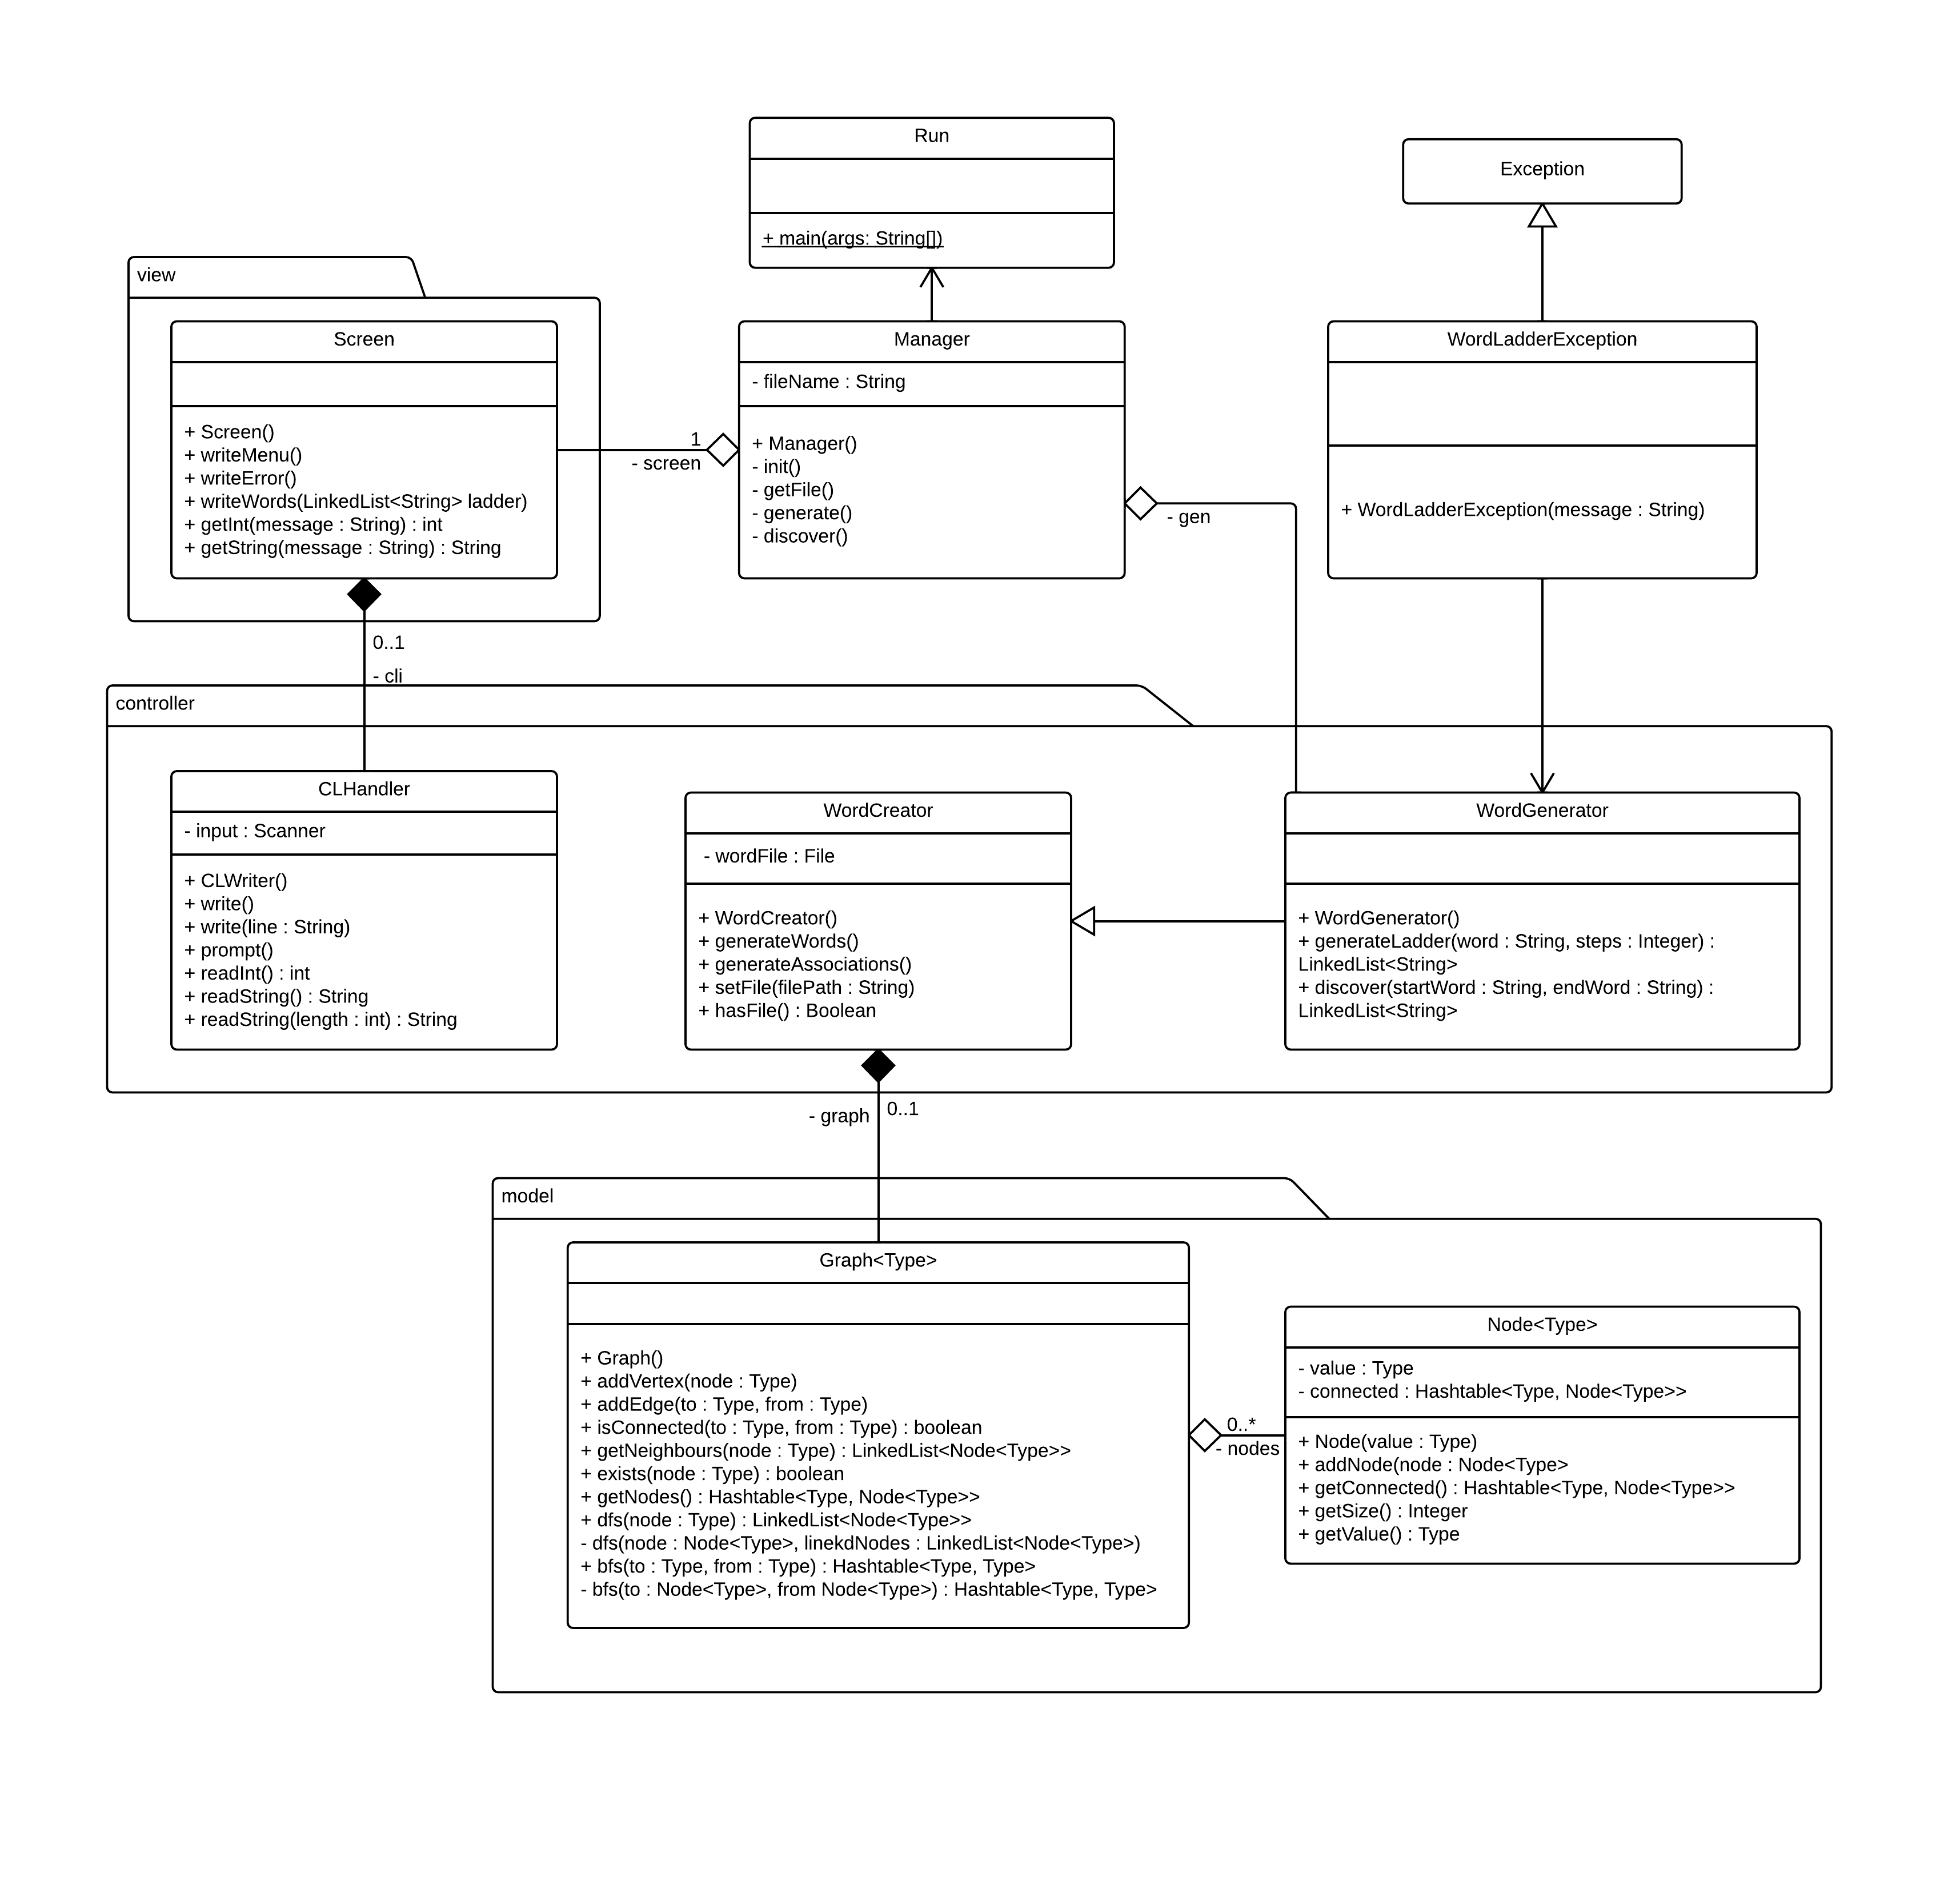
\includegraphics[width=1.66\textwidth,height=1.66\textheight,keepaspectratio]{./images/classdiagram.png}

\section{Justification of classes}

\subsection{Model}

The \texttt{Graph} class is the main data structure for handling all the data, by adding all the words as vertices (or \texttt{Nodes}) when reading the words into the program. I also implemented two different search algorithms (Depth-first search and Breadth-first search) to tackle the two different problems which were set out in the assignment brief. I used the Depth-first search to tackle the generation of the word ladder, as it searches blindly down one branch of the graph until all nodes are visited on one branch before moving to the next unexplored branch\footnote{In hindsight, I wish I researched other searching algorithms before going head first in to a Depth first algorithm, as a Depth-limited search would be more efficient in comparison.}. For discovery of a word ladder, I used breadth-first as it was more likely to find the node in a quicker time, due to looking at each node on a level before traversing down the graph. 

The \texttt{Node} class is just a simple data structure which only holds the value of the node, and a hashtable of other connected nodes. I decided not to add weights on the edges, as each node has a constant distance between the neighbouring nodes.

In both classes I also added a generic type, so it would be reusable for other different graphs in the future with minimal modification. 

\subsection{View}

To display and get user input, I used two classes: \texttt{Screen} and \texttt{CLHandler}. \texttt{CLHandler} is a class I wrote in December 2011 for the CS12130 project which I wrote to handle standard user input and output to the command line, with useful functions to get Integers and specific length strings from the user, while being the only class in the program which outputs text to the user. \texttt{Screen} implements \texttt{CLHandler} which formats the data for user readability before displaying. 

\subsection{Controller}

In \texttt{WordCreator}, I handle the main data manipulation of the words, such as populating the hashtable of the words, and generating associations between words. I kept this out of the model classes, as it’s only specific for wordladders in general, and no help for other graph manipulation. I also decided to have the generation of word ladders in a separate class which inherits from \texttt{WordCreator}, so it would be easy to implement different methods without modifying generation


\section{Pseudocode description}

\subsection{Collecting words from files}

\begin{algorithm}[H]
\SetAlgoLined
	\KwData{file name as a string}
	\eIf{file exists on file system} {
		Open file through a buffered reader \\
		\While{get line from opened file} {
			Remove all punctuation \\
			\eIf{position of space character is -1} {
				Create new node in hashtable \\
			} {
				\For{all words in line} {
					Create new node in hashtable\\
				}
			}
		}
		Close file handler\\
	} {
		Return error to user, ask for a different input file\\
	}

\end{algorithm}

\subsection{Creating associations}

\begin{algorithm}[H]
\SetAlgoLined
	\For{each key in the Hashtable} {
		\For{i = Each letter in the key} {
			\For{j = ASCII values for lowercase letters (96 to 122) } {
				Change letter 'i' to character value of 'j' and place in 'tmp'\\
				\If{Key does not exist for 'tmp' in hashtable} {
					First node linked to Second node\\
					Second Node linked to First Node\\
				}
			}
		}
	}
\end{algorithm}

\subsection{Generation of a word ladder}

\begin{algorithm}[H]
\SetAlgoLined
	Add node to list
	\For{each neighbouring nodes} {
		\If{list doesn't contain node} {
			Recursively call with node
		}
	}
\end{algorithm}

\subsection{Discovery of a word ladder}

\begin{algorithm}[H]
\SetAlgoLined
	Create a queue and add first node
	\While{queue is not empty} {
		Remove node from queue
		\For{Neighbouring nodes from dequeued node} {
			Add node to queue
			Add relationship between neighbouring node and start node
		}
	}
\end{algorithm}

\section{Testing}

\section{Evidence of Testing}

\subsection{Generation}

To show the generation of wordladders, I have generated 3, 5 and 7 word ladders in 3 different word lengths.

\subsubsection{4 Letter Wordladders}

\hspace*{0.15in}
\texttt{head -> herd -> hard}\\

\texttt{foot -> boot -> toot -> tolt -> tolu}\\

\texttt{baby -> baba -> caba -> yaba -> yaya -> raya -> rana}\\

\subsubsection{5 letter Wordladders}
\hspace*{0.15in}
\texttt{speed -> speel -> steel}\\

\texttt{spade -> spale -> shale -> share -> shade}\\

\texttt{plane -> plang -> clang -> cling -> clint -> glint -> glink}\\

\subsubsection{6 letter Wordladders}
\hspace*{0.15in}
\texttt{spider -> spader -> sparer}\\

\texttt{damage -> ramage -> rayage -> ravage -> pavage}\\

\texttt{breast -> brewst -> browst -> frowst -> browse -> broose -> groose}\\

\subsection{Discovery}

To show the discovery of word ladders, I have generated a standard ladder transversing from the start word and then back to the start word from the end word, to check if the length would be the same either way.

\subsubsection{4 Letter Wordladders}
\hspace*{0.15in}
\texttt{head -> lead -> load -> lood -> food -> foot}\\

\texttt{baby -> baba -> bara -> bora -> bort -> boat -> brat -> bray -> xray}\\

\texttt{foot -> boot -> boat -> beat -> heat -> head}\\

\subsubsection{5 letter Wordladders}
\hspace*{0.15in}
\texttt{speed -> steed -> stend -> stond -> stone -> shone -> phone -> prone -> probe}\\

\texttt{tripe -> trite -> arite -> axite -> axile -> anile -> ankle -> ankee -> anker -> asker -> aster -> after -> ofter -> offer}\\

\texttt{probe -> prone -> phone -> shone -> scone -> scene -> scend -> spend -> speed}\\


\subsubsection{6 letter Wordladders}	
\hspace*{0.15in}
\texttt{pirate -> parate -> parage -> pavage -> ravage -> ramage -> damage}\\

\texttt{potato -> potate -> rotate -> rutate -> rugate -> jugate -> jugale -> juggle -> guggle -> gurgle -> burgle -> burgee -> bargee -> barger -> barrer -> barret -> garret -> garrot -> carrot}\\

\texttt{damage -> ramage -> ravage -> pavage -> parage -> parate -> pirate}\\


\section{Evaluation}

\end{document}